%% bare_conf.tex
%% V1.3
%% 2007/01/11
%% by Michael Shell
%% See:
%% http://www.michaelshell.org/
%% for current contact information.
%%
%% This is a skeleton file demonstrating the use of IEEEtran.cls
%% (requires IEEEtran.cls version 1.7 or later) with an IEEE conference paper.
%%
%% Support sites:
%% http://www.michaelshell.org/tex/ieeetran/
%% http://www.ctan.org/tex-archive/macros/latex/contrib/IEEEtran/
%% and
%% http://www.ieee.org/

%%*************************************************************************
%% Legal Notice:
%% This code is offered as-is without any warranty either expressed or
%% implied; without even the implied warranty of MERCHANTABILITY or
%% FITNESS FOR A PARTICULAR PURPOSE!
%% User assumes all risk.
%% In no event shall IEEE or any contributor to this code be liable for
%% any damages or losses, including, but not limited to, incidental,
%% consequential, or any other damages, resulting from the use or misuse
%% of any information contained here.
%%
%% All comments are the opinions of their respective authors and are not
%% necessarily endorsed by the IEEE.
%%
%% This work is distributed under the LaTeX Project Public License (LPPL)
%% ( http://www.latex-project.org/ ) version 1.3, and may be freely used,
%% distributed and modified. A copy of the LPPL, version 1.3, is included
%% in the base LaTeX documentation of all distributions of LaTeX released
%% 2003/12/01 or later.
%% Retain all contribution notices and credits.
%% ** Modified files should be clearly indicated as such, including  **
%% ** renaming them and changing author support contact information. **
%%
%% File list of work: IEEEtran.cls, IEEEtran_HOWTO.pdf, bare_adv.tex,
%%                    bare_conf.tex, bare_jrnl.tex, bare_jrnl_compsoc.tex
%%*************************************************************************

% *** Authors should verify (and, if needed, correct) their LaTeX system  ***
% *** with the testflow diagnostic prior to trusting their LaTeX platform ***
% *** with production work. IEEE's font choices can trigger bugs that do  ***
% *** not appear when using other class files.                            ***
% The testflow support page is at:
% http://www.michaelshell.org/tex/testflow/

% Note that the a4paper option is mainly intended so that authors in
% countries using A4 can easily print to A4 and see how their papers will
% look in print - the typesetting of the document will not typically be
% affected with changes in paper size (but the bottom and side margins will).
% Use the testflow package mentioned above to verify correct handling of
% both paper sizes by the user's LaTeX system.
%
% Also note that the "draftcls" or "draftclsnofoot", not "draft", option
% should be used if it is desired that the figures are to be displayed in
% draft mode.
%
\documentclass[10pt, conference, compsocconf]{IEEEtran}
% Add the compsocconf option for Computer Society conferences.
%
% If IEEEtran.cls has not been installed into the LaTeX system files,
% manually specify the path to it like:
% \documentclass[conference]{../sty/IEEEtran}

% Some very useful LaTeX packages include:
% (uncomment the ones you want to load)

% *** MISC UTILITY PACKAGES ***
%
%\usepackage{ifpdf}
% Heiko Oberdiek's ifpdf.sty is very useful if you need conditional
% compilation based on whether the output is pdf or dvi.
% usage:
% \ifpdf
%   % pdf code
% \else
%   % dvi code
% \fi
% The latest version of ifpdf.sty can be obtained from:
% http://www.ctan.org/tex-archive/macros/latex/contrib/oberdiek/
% Also, note that IEEEtran.cls V1.7 and later provides a builtin
% \ifCLASSINFOpdf conditional that works the same way.
% When switching from latex to pdflatex and vice-versa, the compiler may
% have to be run twice to clear warning/error messages.

% *** CITATION PACKAGES ***
%
\usepackage{cite}
% cite.sty was written by Donald Arseneau
% V1.6 and later of IEEEtran pre-defines the format of the cite.sty package
% \cite{} output to follow that of IEEE. Loading the cite package will
% result in citation numbers being automatically sorted and properly
% "compressed/ranged". e.g., [1], [9], [2], [7], [5], [6] without using
% cite.sty will become [1], [2], [5]--[7], [9] using cite.sty. cite.sty's
% \cite will automatically add leading space, if needed. Use cite.sty's
% noadjust option (cite.sty V3.8 and later) if you want to turn this off.
% cite.sty is already installed on most LaTeX systems. Be sure and use
% version 4.0 (2003-05-27) and later if using hyperref.sty. cite.sty does
% not currently provide for hyperlinked citations.
% The latest version can be obtained at:
% http://www.ctan.org/tex-archive/macros/latex/contrib/cite/
% The documentation is contained in the cite.sty file itself.

% *** GRAPHICS RELATED PACKAGES ***
%
\ifCLASSINFOpdf
   \usepackage[pdftex]{graphicx}
  % declare the path(s) where your graphic files are
   \graphicspath{{./images/}}
  % and their extensions so you won't have to specify these with
  % every instance of \includegraphics
   \DeclareGraphicsExtensions{.pdf,.jpeg,.png}
\else
  % or other class option (dvipsone, dvipdf, if not using dvips). graphicx
  % will default to the driver specified in the system graphics.cfg if no
  % driver is specified.
  % \usepackage[dvips]{graphicx}
  % declare the path(s) where your graphic files are
  % \graphicspath{{../eps/}}
  % and their extensions so you won't have to specify these with
  % every instance of \includegraphics
  % \DeclareGraphicsExtensions{.eps}
\fi
% graphicx was written by David Carlisle and Sebastian Rahtz. It is
% required if you want graphics, photos, etc. graphicx.sty is already
% installed on most LaTeX systems. The latest version and documentation can
% be obtained at:
% http://www.ctan.org/tex-archive/macros/latex/required/graphics/
% Another good source of documentation is "Using Imported Graphics in
% LaTeX2e" by Keith Reckdahl which can be found as epslatex.ps or
% epslatex.pdf at: http://www.ctan.org/tex-archive/info/
%
% latex, and pdflatex in dvi mode, support graphics in encapsulated
% postscript (.eps) format. pdflatex in pdf mode supports graphics
% in .pdf, .jpeg, .png and .mps (metapost) formats. Users should ensure
% that all non-photo figures use a vector format (.eps, .pdf, .mps) and
% not a bitmapped formats (.jpeg, .png). IEEE frowns on bitmapped formats
% which can result in "jaggedy"/blurry rendering of lines and letters as
% well as large increases in file sizes.
%
% You can find documentation about the pdfTeX application at:
% http://www.tug.org/applications/pdftex

% *** MATH PACKAGES ***
%
\usepackage[cmex10]{amsmath}
% A popular package from the American Mathematical Society that provides
% many useful and powerful commands for dealing with mathematics. If using
% it, be sure to load this package with the cmex10 option to ensure that
% only type 1 fonts will utilized at all point sizes. Without this option,
% it is possible that some math symbols, particularly those within
% footnotes, will be rendered in bitmap form which will result in a
% document that can not be IEEE Xplore compliant!
%
% Also, note that the amsmath package sets \interdisplaylinepenalty to 10000
% thus preventing page breaks from occurring within multiline equations. Use:
%\interdisplaylinepenalty=2500
% after loading amsmath to restore such page breaks as IEEEtran.cls normally
% does. amsmath.sty is already installed on most LaTeX systems. The latest
% version and documentation can be obtained at:
% http://www.ctan.org/tex-archive/macros/latex/required/amslatex/math/

% *** SPECIALIZED LIST PACKAGES ***
%
\usepackage{algorithm}
\usepackage{algorithmic}
% algorithmic.sty was written by Peter Williams and Rogerio Brito.
% This package provides an algorithmic environment fo describing algorithms.
% You can use the algorithmic environment in-text or within a figure
% environment to provide for a floating algorithm. Do NOT use the algorithm
% floating environment provided by algorithm.sty (by the same authors) or
% algorithm2e.sty (by Christophe Fiorio) as IEEE does not use dedicated
% algorithm float types and packages that provide these will not provide
% correct IEEE style captions. The latest version and documentation of
% algorithmic.sty can be obtained at:
% http://www.ctan.org/tex-archive/macros/latex/contrib/algorithms/
% There is also a support site at:
% http://algorithms.berlios.de/index.html
% Also of interest may be the (relatively newer and more customizable)
% algorithmicx.sty package by Szasz Janos:
% http://www.ctan.org/tex-archive/macros/latex/contrib/algorithmicx/

% *** ALIGNMENT PACKAGES ***
%
%\usepackage{array}
% Frank Mittelbach's and David Carlisle's array.sty patches and improves
% the standard LaTeX2e array and tabular environments to provide better
% appearance and additional user controls. As the default LaTeX2e table
% generation code is lacking to the point of almost being broken with
% respect to the quality of the end results, all users are strongly
% advised to use an enhanced (at the very least that provided by array.sty)
% set of table tools. array.sty is already installed on most systems. The
% latest version and documentation can be obtained at:
% http://www.ctan.org/tex-archive/macros/latex/required/tools/

%\usepackage{mdwmath}
%\usepackage{mdwtab}
% Also highly recommended is Mark Wooding's extremely powerful MDW tools,
% especially mdwmath.sty and mdwtab.sty which are used to format equations
% and tables, respectively. The MDWtools set is already installed on most
% LaTeX systems. The lastest version and documentation is available at:
% http://www.ctan.org/tex-archive/macros/latex/contrib/mdwtools/

% IEEEtran contains the IEEEeqnarray family of commands that can be used to
% generate multiline equations as well as matrices, tables, etc., of high
% quality.

%\usepackage{eqparbox}
% Also of notable interest is Scott Pakin's eqparbox package for creating
% (automatically sized) equal width boxes - aka "natural width parboxes".
% Available at:
% http://www.ctan.org/tex-archive/macros/latex/contrib/eqparbox/

% *** SUBFIGURE PACKAGES ***
%\usepackage[tight,footnotesize]{subfigure}
% subfigure.sty was written by Steven Douglas Cochran. This package makes it
% easy to put subfigures in your figures. e.g., "Figure 1a and 1b". For IEEE
% work, it is a good idea to load it with the tight package option to reduce
% the amount of white space around the subfigures. subfigure.sty is already
% installed on most LaTeX systems. The latest version and documentation can
% be obtained at:
% http://www.ctan.org/tex-archive/obsolete/macros/latex/contrib/subfigure/
% subfigure.sty has been superceeded by subfig.sty.

%\usepackage[caption=false]{caption}
%\usepackage[font=footnotesize]{subfig}
% subfig.sty, also written by Steven Douglas Cochran, is the modern
% replacement for subfigure.sty. However, subfig.sty requires and
% automatically loads Axel Sommerfeldt's caption.sty which will override
% IEEEtran.cls handling of captions and this will result in nonIEEE style
% figure/table captions. To prevent this problem, be sure and preload
% caption.sty with its "caption=false" package option. This is will preserve
% IEEEtran.cls handing of captions. Version 1.3 (2005/06/28) and later
% (recommended due to many improvements over 1.2) of subfig.sty supports
% the caption=false option directly:
%\usepackage[caption=false,font=footnotesize]{subfig}
%
% The latest version and documentation can be obtained at:
% http://www.ctan.org/tex-archive/macros/latex/contrib/subfig/
% The latest version and documentation of caption.sty can be obtained at:
% http://www.ctan.org/tex-archive/macros/latex/contrib/caption/

% *** FLOAT PACKAGES ***
%
%\usepackage{fixltx2e}
% fixltx2e, the successor to the earlier fix2col.sty, was written by
% Frank Mittelbach and David Carlisle. This package corrects a few problems
% in the LaTeX2e kernel, the most notable of which is that in current
% LaTeX2e releases, the ordering of single and double column floats is not
% guaranteed to be preserved. Thus, an unpatched LaTeX2e can allow a
% single column figure to be placed prior to an earlier double column
% figure. The latest version and documentation can be found at:
% http://www.ctan.org/tex-archive/macros/latex/base/

%\usepackage{stfloats}
% stfloats.sty was written by Sigitas Tolusis. This package gives LaTeX2e
% the ability to do double column floats at the bottom of the page as well
% as the top. (e.g., "\begin{figure*}[!b]" is not normally possible in
% LaTeX2e). It also provides a command:
%\fnbelowfloat
% to enable the placement of footnotes below bottom floats (the standard
% LaTeX2e kernel puts them above bottom floats). This is an invasive package
% which rewrites many portions of the LaTeX2e float routines. It may not work
% with other packages that modify the LaTeX2e float routines. The latest
% version and documentation can be obtained at:
% http://www.ctan.org/tex-archive/macros/latex/contrib/sttools/
% Documentation is contained in the stfloats.sty comments as well as in the
% presfull.pdf file. Do not use the stfloats baselinefloat ability as IEEE
% does not allow \baselineskip to stretch. Authors submitting work to the
% IEEE should note that IEEE rarely uses double column equations and
% that authors should try to avoid such use. Do not be tempted to use the
% cuted.sty or midfloat.sty packages (also by Sigitas Tolusis) as IEEE does
% not format its papers in such ways.

% *** PDF, URL AND HYPERLINK PACKAGES ***
%
%\usepackage{url}
% url.sty was written by Donald Arseneau. It provides better support for
% handling and breaking URLs. url.sty is already installed on most LaTeX
% systems. The latest version can be obtained at:
% http://www.ctan.org/tex-archive/macros/latex/contrib/misc/
% Read the url.sty source comments for usage information. Basically,
% \url{my_url_here}.

\usepackage{color}

% *** Do not adjust lengths that control margins, column widths, etc. ***
% *** Do not use packages that alter fonts (such as pslatex).         ***
% There should be no need to do such things with IEEEtran.cls V1.6 and later.
% (Unless specifically asked to do so by the journal or conference you plan
% to submit to, of course. )


% correct bad hyphenation here
\hyphenation{op-tical net-works semi-conduc-tor}

\begin{document}
% use linebreaks \\ within to get better formatting as desired
\title{Scalable Parallel Tracking of Time-Varying 3D Flow Features}

% author names and affiliations
% use a multiple column layout for up to two different
% affiliations

\author {
\IEEEauthorblockN{Authors Name/s per 2nd Affiliation (Author)}
\IEEEauthorblockA{line 1 (of Affiliation): dept. name of organization\\
line 2: name of organization, acronyms acceptable\\
line 3: City, Country\\
line 4: Email: name@xyz.com}
\and
\IEEEauthorblockN{Authors Name/s per 2nd Affiliation (Author)}
\IEEEauthorblockA{line 1 (of Affiliation): dept. name of organization\\
line 2: name of organization, acronyms acceptable\\
line 3: City, Country\\
line 4: Email: name@xyz.com}
}

% make the title area
\maketitle

\begin{abstract}
Large-scale time-varying volumetric data set can take terabytes to petabytes of storage space to store and process. One promising approach is to process the data in parallel in situ or batch, extract features of interest and analyze only those features, to reduce required memory space by several orders of magnitude for the following visualization tasks. However, extracting volumetric features in parallel is a non-trivial task as features might span over multiple processors, and local partial features can be only visible within their own processor. In this paper, we discuss how to generate and maintain connectivity information of features across different processors. Based on this connectivity information, partial features can be integrated, which makes possible for the large-scale feature extraction and tracking in parallel. We demonstrate the effectiveness and scalability of different approaches on two data sets, and discuss the pros and cons of each approach.

\end{abstract}

\begin{IEEEkeywords}
feature tracking; parallel graph;
\end{IEEEkeywords}

% For peer review papers, you can put extra information on the cover
% page as needed:
% \ifCLASSOPTIONpeerreview
% \begin{center} \bfseries EDICS Category: 3-BBND \end{center}
% \fi
%
% For peerreview papers, this IEEEtran command inserts a page break and
% creates the second title. It will be ignored for other modes.
\IEEEpeerreviewmaketitle

\section{Introduction}
The accessibility to supercomputers with increasing computing power has enabled scientists to simulate physical phenomena of unprecedented complexity and resolution. However, these large-scale time-varying data sets can take giga- or even tera-bytes of space to preserve. One promising solution to the problem is to introduce feature extraction and tracking techniques. Instead of duplicating raw data along the exploring process, dealing with features of interest typically requires memory space that is several orders of magnitude smaller than the raw data.

However, large vortical data sets are typically presented and processed in a distributed fashion simply because of the shear size. Extracting and tracking features embedded in a distributed vortical data set is a non-trivial task. Existing researches on feature-based data visualization have been done mostly focusing on decomposing features using quantitative measures such as size, location, shape or topology information, and so on. These measures cannot be applied to distributed volume data directly since vortical features consist of certain amount of voxels and are very likely to span over distributed data blocks as they evolve over time. Therefore existing quantitative measures of partial data scattered across different data blocks cannot be used to describe an integrated feature, unless the distribution of partial features can be obtained beforehand.

To obtain the distribution information of features, a connectivity map of each feature should be generated and maintained. In this paper, we propose an approach to creating and maintaining feature residual information as well as connectivity information using parallel graphs. Comparing to the existing approaches, which generate and maintain the global feature information in a single host node, our approach can be done locally that only involves residual data blocks of target features. This requires least communication overhead and avoids the potential link contention. We demonstrate the effectiveness of this method with three vortical flow data sets and the scalability of our system in a distributed environment.

\section{Related Work}
\subsection{Parallel Feature Extraction and Tracking}
Extraction and tracking are two closely related problems in feature-based visualization. Although many feature tracking algorithms have been introduced, most of them extract features from individual time steps and then try to associate them between consecutive time steps. Silver and Wang \cite{Silver1997} defined threshold connected components as their features, and tracked overlapped features between successive time steps by calculating their differences. Octree was employed in their method to speed up the performance and the criteria they used were domain dependent. Reinders et al. \cite{Reinders2001} introduced a prediction verification tracking technique that calculates a prediction by linear extrapolation based on the previous feature path, and a candidate will be added to the path if it corresponds to that prediction. Ji and Shen \cite{Ji2003} introduced a method to track local features from time-varying data by using higher-dimensional iso-surfacing. They also used a global optimization correspondence algorithm to improve the robustness of feature tracking \cite{Ji2006}. Caban et al. \cite{Caban2007} estimated a tracking window and then tried to find the best match between that window and different sub-volumes of subsequence frames by comparing their distance of textural properties. Also, Bremer et al. \cite{Bremer2007} described two topological feature tracking methods, one employs Jacobi sets to track critical points while the other uses distance measures on graphs to track channel structures.

Most of the aforementioned methods extract features from each time step independently and then apply correspondence calculations. This could become very slow when the data size become relatively large. Muelder and Ma \cite{Muelder2009} proposed a prediction-correction approach that first predicts feature region based on the centroid location of that in previous time steps, and then corrects the predicted region by adjusting the surface boundaries via region growing and shrinking. This approach is appealing because of its computing efficiency and the reliability in an interactive system.

To boost up the speed for feature tracking in data-distributed applications, Chen and Silver \cite{Chen2003} introduced a two stage partial-merge strategy using master-slave paradigm. The slaves first exchange local connectivity information using Binary-tree merge, and then a visualization host collects and correlates the local information to generate the global connectivity. This approach is not scalable since half of the processors will become idle after each merge. It is also unclear how the visualization host can efficiently collect local connectivity information from non-server processors, since gathering operation is typically very expensive given a large number of processors. 

The approach proposed in this paper follows a different strategy. Instead of being sent back to a host, the local connective information is computed and preserved only in the nodes where correspondent features reside. Hence there is no global connectivity information preserved in the host, and the host only serves as an interface to broadcast the criterion of feature of interest to the other nodes. In this way, the computation of merging local connectivity information is distributed to the slaves and thus effectively reduces the potential communication bottleneck on the host.

Moreover, our approach does not need a global synchronization for gathering all local connectivity information at the host, hence avoids potentially long computation time caused by features spanning over a large number of nodes. In addition, there are no needs to set a barrier to wait for all connectivity information being sent back to the host and thus if there exists features that span over a large number of nodes but was not selected by the user, the potentially long computation time for these features will not block the whole process. This makes it ideal for an interactive system, where users can select the features of interest and instantly receive the visual feedback as the features evolves.

\subsection{Parallel Graph Algorithm and Applications}
Graph-based algorithms have long been studied and used for a wide range of applications, typically along the line of divide-and-conquer approaches. Researches have been done on 

Grundmann et al. \cite{Grundmann2010} recently proposed a hierarchical graph-based approach for video segmentation, a closely related research topic to 3D flow feature extraction as video can be treated as a space-time volume of image data \cite{Klein2002}. In their work, a connected sequence of time-axis-aligned subsets of cubic image volumes are assigned to a set of corresponding processors, and incident regions are merged only if they are inside the volumes window. Incident regions on window boundary, however, are first marked as ambiguous and later connected by merging neighboring window to a larger one that consists of the unresolved regions form both window on their common boundary. This approach is not applicable if the utilization the memory space of each processing unit is the main concern such that the allocated volume size before merging already reaches the capacity. Same restriction applies to the parallelized BK algorithm \cite{Boykov2004} proposed by Liu and Sun \cite{Liu2010}, in which data are uniformly partitioned and then adaptively merged to achieve fast graph-cuts. These approaches are suitable for shared-memory but not message-passing parallelization as for their frequent shifting on data ranges.

\section{Algorithm Design}
Though features can be extracted within individual processors using the conventional methods, they might also span over multiple data blocks, which is unavoidable as the number of processors increases. To extract and trace a feature over a distributed volume data set, we need to build and maintain the connectivity information of the feature across multiple nodes. As feature descriptors, such as size, curvature, and velocity, are distributed among processors, connectivity information can facilitate us to obtain the description of a feature from neighboring processors, and enable more advanced operations such as similarity evaluation.
%makes it possible to gather from each part of the feature resides in different processors these descriptions such that feature tracking or and similarity test could be achieved.
However, it typically requires data exchanges among processors to build and maintain the connectivity information, and thus incurs extra communication cost. To design a proper communication scheme for better performance and scalability, we carefully consider the following three factors in our design:

\begin{itemize}
\item How many communications are required to complete the connectivity graph;
\item How many processors will be involved in one communication;
\item How much data will be sent and received in one communication.
\end{itemize}

In the following sections, we will give a detailed description on how to build and maintain such connectivity information using an undirected unweighted graph to minimize the cost over the above three factors.

\subsection{Feature Extraction}
Feature extraction is a process that first detects a feature, and then calculates quantitative attributes characterizing the feature. In general, a feature can be any interesting pattern, structure, or object that is considered relevant for investigation. In our application, a feature is defined as the collection of voxices encompassed by a certain iso-surface. Such a volumetric feature could be extracted by conventional techniques such as region growing, geometry or topology based clustering, or other domain specific algorithms as described in [] [] [] [].

In our work, we use a standard region-growing algorithm [14] to partition the original volume data into an initial set of features. This can be done by first spreading a set of seeding points inside the volume, and then clustering voxices into separate regions. Each region is regarded as a single feature. Usually, scientists prefer to focus on features that are meaningful as dictated by their underlying research studies. Potential features detected by the region-growing algorithm, however, are often cluttered and contain noise, which might be far from expected. Therefore, an iterative refinement process is conventionally applied to improve the results after the potential feature set being generated. On the other hand, we note that the refinement process can typically reduce the number of features, which also can lower computational cost of tracking.

Tangelder and Veltkamp [27] presented the applicability and performance of context-based 3D shape descriptors and the corresponding retrieval methods. Their work suggested that when designing an interactive refinement process, we need to carefully select a set of feature descriptors, which should be deformation robust, such as size, location, or skeletal curvature. In addition, we also need to consider computational efficient in our design. 
%Based on the discussion in their work, we can characterize the interactive refinement process as primarily concerned with those computationally efficient yet with significant discriminating deformation robust descriptors, such as size, location, or skeletal curvature. 
After specific features have been identified from a single time step, we can track their evolution over time using a prediction-correction approach. The feature locations in a future time step can be predicted from the location of features in the previous time steps. Once prediction is made, the actual region can be obtained by adjusting the surface of the predicted region: first shrink the edge surface points to obtain the mutual region between consecutive time steps, and then use of a region-growing method to generate the refined region.

This prediction-correction approach was proved effective and efficient for tracking feature on a single processor [32]. However, when the size of the volume data becomes too large to be fit into one processor, a cluster of multiple processors are often needed to process the data in parallel. One challenge to parallelize the tracking approach lies in that it can be difficult to obtain the global feature descriptions unless they can be shared and merged in an efficient way. This is because volumetric features may span over multiple processors and partial features on different nodes are operated independently.

An intuitive way of exchanging such feature information is first to find how features span over multiple processors, and then to merge feature descriptions according to the connectivity information.

\subsection{Creating Partial Connectivity Graph}
If we partition a volumetric data set into the blocks across a regular processor grid, it is very likely that some features can cross multiple processors and blocks. We note that the cross-section of such a feature on the boundary of two adjacent blocks should match. Leveraging this property, we could connect separate parts of a feature on the adjacent data blocks by comparing their sections on the correspondent boundary surface.

Since data is distributed, each processor is not aware of the partial features identified on the other processors. Exchanging the voxels on the sectional area between two adjacent processors would be sufficient for finding the possible matches of partial features between these two processors. However, we choose to exchange more abstract data, that is the minimal and maximal (min-max) coordinate values and the geometric centroid of the cross-sectional area, to reduce the amount of data exchanged over network. The min-max coordinate values are not optional because they ensure correct connectivity for some special cases where one cross-sectional area is surrounded by another concave or hollow area whose centroid points happen to be the same, as depicted in Figure~\ref{fig:special}.

\begin{figure}[ht]
\centering
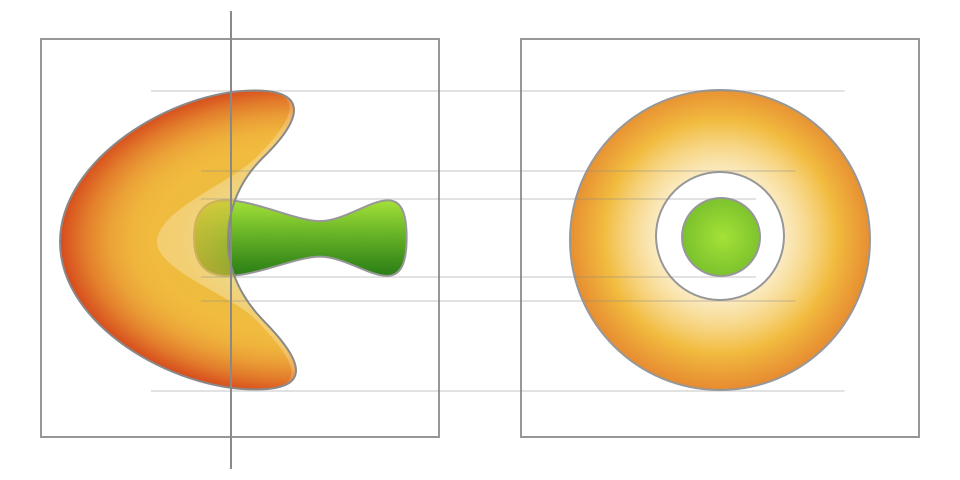
\includegraphics[width=0.9\linewidth]{figure1@2x.png}
\caption{A special case where two features share a same centroid on the section.}
\label{fig:special}
\end{figure}

A voxel-width ``ghost surface" that stores boundary surface belonging to neighboring blocks might help to achieve voxel-wise matching for partial features. However, 
%for non-post-processing situation where data set are not pre-determined, 
maintaining such ghost surfaces requires frequent inter-process communication and is considerably expensive for data generated in real-time. 
%Instead, a ±1 voxel tolerance was given in our work when trying to match two geometric centroid points on the boundary surfaces. That is, if the neighboring centroid is within the eight direct neighbor of the domestic centroid, they are considered a match and the two separated parts were belong to the same feature.
Instead, we use a simplified approach which requires much less communication cost. That is, if the spatial distance between two centroid points of two neighboring partial features is less than two voxels, the two features are considered a match and belong to the same feature.

The creation of partial connectivity graph will not introduce extra computation cost as it can be done along with the direction of region growing. A new edge is appended to the existing graph when a local feature touches the block boundary.
%taking the ID of the target block that shares a same boundary surface as the ending vertex, as well as the global index of the centroid points as edge value.
In the graph, the new edge connects one existing block with the new detected block of a feature. The ending vertices of an edge is denoted using the block indices. Thus the ID of the new detected block is assigned as one ending vertex of the new edge. In addition, the global index of the centroid point is assigned as the edge value. 

Algorithm~\ref{alg:local} shows the detailed algorithm of creating local partial connectivity graph.
%------------------------------------------------
\begin{algorithm}
\caption{Creating Partial Connectivity Graph}
\label{alg:local}
\begin{algorithmic}[1]
\STATE $edgeList \leftarrow new List()$
\STATE $featureList \leftarrow new List()$
\IF{Current time step $t = t0$}
	\STATE // Initialize random seeding points
	\STATE $seedList \leftarrow randomVortices()$
	\FOR {each $seed$ in $seedList$}
		\STATE $feture \leftarrow expendRegion()$
		\STATE append $feture$ to $featureList$
	\ENDFOR	
\ELSE
	\FOR {each $feture$ in $featureList$}
		\STATE $feture \leftarrow predictRegion()$
		\STATE $feture \leftarrow adjustRegion()$	
		
		\STATE $start \leftarrow$ current processor ID
		\STATE $end \leftarrow$ target neighboring processor ID
		\STATE $min,max \leftarrow$ min-max boundary coordinate
		\STATE $index \leftarrow$ global voxel index of centroid
		\STATE Edge $e = Edge(start, end, min, max, index)$
		\STATE append $e$ to $edgeList$
	\ENDFOR
\ENDIF
\end{algorithmic}
\begin{algorithmic} \STATE \end{algorithmic}	% line separator
\begin{algorithmic}[1]
\STATE $adjustRegion()$
	\IF{Voxel $v$ on boundary surface}
		\STATE $updateMixMaxBoundary()$
		\STATE $updateBoundaryCentroid()$
	\ENDIF
\end{algorithmic}
\end{algorithm}
%------------------------------------------------

\textcolor{red}{
// TODO (put to result, performance analyze)
Memory cost, each feature on boundary will use two INTs, 1 as global centroids coordinate, the other as target node number. even if there's 1000 features on the boundary, it would cost more than 1000 * 5 * 4 = 20mb to store this graph, neglectable compare to the volume data itself. (But kind of large if used for communication)
}

\subsection{Creating Global Connectivity Graph}
\subsubsection{The naive solution}
%To construct the global description of a partitioned feature, local connectivity graphs need to be merged with those derived from their neighboring processors, after they were individually created. A naive approach to gather local connectivity graphs is to send all edges sharing the same ending vertex to that target processor, and to merge edges sent from neighboring processor. Two edges are merged if they suffice the following three condition:

Local connectivity graphs need to be merged to construct the global description of a partitioned feature. A naive approach to gathering local connectivity graphs is to let each processor exchanges the shared edges with its neighbors. After exchanges, two edges are merged at a processor if they satisfy the following three conditions:

\begin{itemize}
\item The starting and ending vertices are reversely matched;
\item The min-max boundary coordinate do match;
\item Edge centroid is located within direct neighbors.
\end{itemize}

Recall that the starting vertex of an edge represents the current processor ID, and the ending vertex represents the ID of a neighboring processor whose partial feature is adjacent to the local one. The edge value represents the global coordinate of the geometric centroid and the min-max boundary on the shared boundary surface. If two edges match to each other, the two partial features must share a same boundary section with the same centroid and section region. In other word, these two partial features are resulted by partitioning a original feature, and should be considered the same feature sharing a same feature ID.

Algorithm~\ref{alg:merge} shows the detailed process to merge matched edges (henceforth referred to as \emph{REDUCE}).
%------------------------------------------------
\begin{algorithm}
\caption{REDUCE: Merging Matched Edges}
\label{alg:merge}
\begin{algorithmic}[1]
\REQUIRE $localEdges$, $recievedEdges$
\FOR {each $ei$ in $localEdges$}
	\FOR {each $ej$ in $recievedEdges$}
		\IF{$ei.start$ = $ej.end$ and $ej.start$ = $ei.end$ \textbf{and}
			$ei.min$ = $ej.min$ and $ei.max$ = $ej.max $ \textbf{and}
			$ei.centroid \approx ej.centroid$}
			\IF {$ei.id < ej.id$}
				\STATE $ej.id \leftarrow ei.id$
			\ELSE
				\STATE $ei.id \leftarrow ej.id$
			\ENDIF
		\ENDIF
	\ENDFOR	
\ENDFOR	
\end{algorithmic}
\end{algorithm}
%------------------------------------------------

This naive solution may work for data sets with small features. However, if there are long curly features partitioned evenly over the process grid,
%In order to gather and merge the whole feature, each processor needs to talk to its neighbors and spread the edge exchange operation one by one like that in the "telephone" game.
each processor needs to consecutively communicate with its neighbors to inclemently gather and merge a global feature. 
This requires O(${N_p}$) communications to connect a single feature, where ${N_p}$ is the number of processors in the grid. Consequently, the total communication cost is O(${N_f \times N_p}$) times communication, where ${N_f}$ is the number of features within one time step. In addition, since one processor cannot predict how many edges it will receive from its adjacent processors, it is hard to schedule the communication process.

\subsubsection{The centralized approach}
A possible solution is to use a master-slave hierarchy to reduce the number of communication required for merging all edges. The master-slave hierarchy can be constructed using a separate host processor. %When the feature extraction process is done, local connectivity graphs with edges representing how many features have touched the block boundary as well as where they are located on the surface within each individual processor will be gathered to the host processor. 
When the feature extraction process is done, the edges of a local graph represents the number of features across the block boundary, and also encodes the location information of each local feature. All local graphs are then gathered to the host processor. 
After this \emph{Gather} operation is done, that is the host processor has collected all local graphs, the REDUCE operation starts to merge the edges from each partial graph to construct a single global connectivity graph.

The merit of this centralized approach lies in that it requires inter-processor communication only once. 
%What is more, a global graph of feature information could be preserved in the host processor, which makes it easy for the host to response directly without pulling information from slave processors a second time. 
Moreover, the global graph of feature information can be preserved in the host, and the host can response feature queries directly without pulling information the slaves again. 
%However the drawback of this approach is also obvious. Since all partial connectivity graphs preserved in each processor will be sent to a single processor, there exists potential bottlenecks, both communication and computational, on the host processor.
However, this approach has an obvious drawback. Since all partial graphs are sent to the host, there exists potential bottlenecks, both in communication and computation, on the host.  

\subsubsection{The decentralized approach}
A better solution is to decentralize from REDUCE on a single host processor to all processors that are available. After the feature extraction process is done and so does the creation of local connectivity graphs, an \emph{Allgather} process starts to exchange all local connectivity graphs within each processor to all the others. Each processor will first collect a full copy of all local connectivity graphs followed by the same REDUCE process to merge the edges into a single concise connectivity graph.

\begin{figure}[ht]
\centering
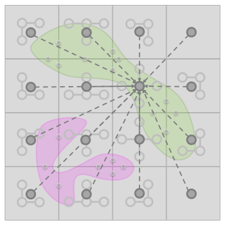
\includegraphics[width=0.45\linewidth]{figure3.png}
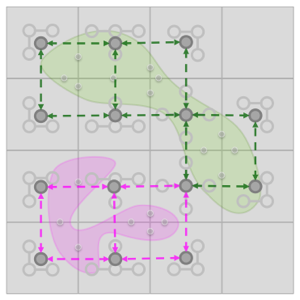
\includegraphics[width=0.45\linewidth]{figure4.png}
\caption{Left: each processor gather partial graphs from all the other processors; Right: a special case where two features share a same centroid.}
\label{fig:decent}
\end{figure}

\marginpar{\textcolor{red}{where is the figure~\ref{fig:decent} referred?}}

Though the ``redundant" host processor is no more required when applying for computation resources, this approach does not actually solve the bottleneck problem since now every processor is now acting like a host since they still need to gather all partial graphs and try merging them together. For real world data set, however, it is rarely the case that a single feature will span over every processor. In other word, it is unnecessary for a processor to gather edges of features that are not local. To reduce the redundant communications with every other processor in the grid, the decentralized approach could be further improved such that we only consider those processors that are directly adjacent to the current one. That is, each processor only talks to its direct neighbors and shares information with them regardless what is happening outside.

For a regularly partitioned volumetric data set, there are at most six direct neighbors for each processor. Instead of gathering connectivity information from all other processors in the grid, each processor only gathers local graphs of neighboring processors. This could be considered as a higher level of region growing, which starts from one seeding processor and then grows to its adjacent processors by exchanging and merging connectivity information in a bread-first fashion until all cross-boundary features are connected.

The detailed scheduling algorithm is depicted in Algorithm~\ref{alg:schedule}.
%------------------------------------------------
\begin{algorithm}
\caption{Processor Level Region Growing}
\label{alg:schedule}
\begin{algorithmic}[1]
\REQUIRE $adjacentProcessors$, $localEdges$
\STATE $toSend, toRecv \leftarrow true$	// init scheduling flags
\STATE $\delta \leftarrow localEdges$	// init data to be sent
\WHILE {$toSend$ = $true$ or $toRecv$ = $true$}
	\STATE $target \leftarrow toRecv$ = $true$ ? $myRank$ : null
	\STATE $procsToSync \leftarrow Allgather(target)$
	\FOR {each $proc$ in $procsToSync$}
		\IF {$toSend$ = $true$}
			\STATE send $\delta$ to $proc$
		\ENDIF
		\IF {$toRecv$ = $true$}
			\STATE receive $\delta\prime$ from $proc$
		\ENDIF
	\ENDFOR
	\STATE $toSend \leftarrow procsToSync$ is empty ? $false$ : $true$
	\STATE $toRecv \leftarrow false$
	\STATE $localEdges \leftarrow Reduce(localEdges, \delta\prime)$
\ENDWHILE
\end{algorithmic}
\begin{algorithmic} \STATE \end{algorithmic}	% line separator
\begin{algorithmic}[1]
\STATE $Reduce(localEdges, \delta\prime)$
	\FOR {each $edge$ in $\delta\prime$}
		\IF {$edge$ is new}
			\STATE add $edge$ to $\delta$
			\STATE $toRecv \leftarrow true$
		\ENDIF
	\ENDFOR	
\end{algorithmic}
\end{algorithm}
%------------------------------------------------

For the worst case that a feature spans over all of the processors, it takes O(C∛(|N|)) time \marginpar{\textcolor{red}{what is this?}} to finish the search for connected processors, much faster than the previous O(N) time for all gathering among all processors.

\subsubsection{The hybrid approach}
We can still take a step further to optimize the aforementioned decentralized approach. As volume data evolves over time, the internal features may vary but should not change drastically in size and shape nor location if the time interval for sampling is sufficiently small. Thus we can apply the prediction-correction approach to further reduce the number of times required to complete the connectivity graph.

\begin{figure}[ht]
\centering
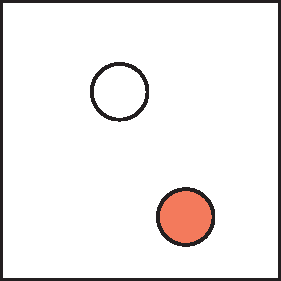
\includegraphics[width=0.45\linewidth]{blank.png}
\caption{}
\label{fig:improve}
\end{figure}

For every time step, $t_i$, when the global connectivity graph is completed, new local communicators will be updated for the next time step, $t_{i+1}$, with the union of processors that share a same edge with the current processor, as shown in Figure~\ref{fig:improve}. However,the edges from these processors are required to complete the global connectivity graph, no matter which approach is used. Hence, for these must-involve processors, we apply the Decentralize-I approach, allowing the minimum one-time synchronization to finish gathering all edges that are necessary for updating the connectivity graph based on the graph created at the previous time step, $t$. Then, the processor-level region growing explained in 3.3.3 is applied to extend the ``boundary" of processes, obtaining newly connected processors caused by the evolution of the original volume. In addition, only those edges that are changed and not synchronized will be sent. This ensure that we minimize the amount of data being sent over network.
The detail algorithm of the hybrid approach is given in Algorithm~\ref{alg:improve}.

%------------------------------------------------
\begin{algorithm}
\caption{TBA}
\label{alg:improve}
\begin{algorithmic}[1]
\STATE	
\end{algorithmic}
\end{algorithm}
%------------------------------------------------

\section{Application}

\subsection{Feature Selection and Refinement}
To allow a user to select or highlight certain features is commonly required in various applications. 
Since the feature extraction is performed independently within each PE, 
%one of the potential function need to be addressed is that how do they know if their adjacent processor was has the feature to be highlighted and whether it has the other part of the features. 
we need to design a method to let each processor know if the features on its adjacent processor are selected or not.  
Intuitively, we can implement this by sending a message to the adjacent PE whenever a feature was detected to touch the surface boundary. But if the target feature spans over multiple PEs, this sending/receiving procedure would take several rounds to end. This is potentially a big problem when the PE/Volume ratio is relatively high such that each feature spans over a lot of PEs. Another problem is that, if a PE has two selected features whose connectivity information arrive in different rounds, it requests to compute twice, which again, will become a problem when PE/Volume ratio is large.

By introducing the global connectivity graph in our approach, whenever part of the feature was selected, the unique feature id will be sent back to the host processor and then be broadcasted to all PEs containing it. Thus, the selection can be finished only in one round.

Based on the coordinates user specified or clicked on the volume rendering result, 
%the residual processor as well as the feature, if the point was included by, could be obtains. 
we can identify the user selected processor and feature.
Then the host processor imply broadcasts the selected feature id to all those processors who has the partial feature to be highlighted.


\subsection{Feature Tracking}
Before you begin to format your paper, first write and save the content as a separate text file. Keep your text and graphic files separate until after the text has been formatted and styled. Do not use hard tabs, and limit use of hard returns to only one return at the end of a paragraph. Do not add any kind of pagination anywhere in the paper. Do not number text heads-the template will do that for you.

Finally, complete content and organizational editing before formatting. Please take note of the following items when proofreading spelling and grammar:

\section{Result}
\subsection{Performance Result}
\subsection{Visualization Result}

\section{Conclusion}
In this paper, we proposed a decentralized approach that all feature connectivity information are created and preserved among distributed processors. Traditional approaches perform connectivity test on each processor and subsequently correspond them in a host processor after gathering all or partially merged connectivity information. Our approach does not follow this paradigm. Rather, %instead of sending local connectivity information back to the host, they are computed and preserved only in processors where correspondent feature resides in. 
instead being sent back to the host, the local connectivity information are computed and preserved only in the local processor. 
There is no copy of the global feature information preserved in the host, and the host only acts as the interface from where the criterion of feature of interest is broadcast. In this way, the computation of merging local connectivity information is distributed to the slaves, which can effectively remove the potential communication bottleneck on the host processor. 
Moreover, there's no need to set a barrier and wait for all connectivity information being sent back to the host, thus if one of the features spans over a large number of processors but was not selected by the user, the potentially long computation time for this feature will not be considered. This makes it ideal for an interactive system, where users can select the feature of interest and instantly receive the visual feedback as the feature evolves. \marginpar{\textcolor{red}{unreadable. it seems to repeat the previous sentences.}}

% use section* for acknowledgement
\section*{Acknowledgment}
The authors would like to thank...
more thanks here

% trigger a \newpage just before the given reference
% number - used to balance the columns on the last page
% adjust value as needed - may need to be readjusted if
% the document is modified later
%\IEEEtriggeratref{8}
% The "triggered" command can be changed if desired:
%\IEEEtriggercmd{\enlargethispage{-5in}}

% references section

\bibliographystyle{IEEEtran}
\bibliography{ipdps_2013}

% <OR> manually copy in the resultant .bbl file
% set second argument of \begin to the number of references
% (used to reserve space for the reference number labels box)
%\begin{thebibliography}{1}
%\end{thebibliography}

\end{document}